% 原文 p.222

\subsectionlink{スピン環境模型}
それでは、調和振動子からなる環境の研究から、環境をスピン$1/2$粒子、すなわち量子二準位系の集合で表す模型の分析へ、焦点を移そう。5.1.2節では、そのようなスピン環境を考える物理的動機と、振動子環境との主要な違いを、すでに論じた。

スピン粒子で表された中心系が、ほかのスピンの集まりに線形に結合する系は、物理的に最も重要で、最もよく研究されたスピン環境模型である。この「スピン・スピン模型」が適する典型的状況は、超伝導量子ビットなどの単一の二準位系が、低温環境に強く結合する場合である（5.1節の議論参照）。もう一つの「標準的」可能性である、
% 原文 p.223
\hypertarget{srcpage:223}{}\label{srcpage:223}
中心調和振動子と二準位系環境との相互作用は、いわゆる量子電気機械系（6.4.2節参照）や、$\mu\mathrm m$尺度のイオントラップ\cite{ref242}でのデコヒーレンスと散逸の研究において、最近ようやく注目され始めた。

本節では、そのようなスピン環境模型の異なる側面を調べる。スピン・スピン模型の議論は、スピン・ボソン模型と同じような構成とする。まず5.4.1節では、2.10節のデコヒーレンス模型を単純に一般化した、スピン・スピン模型を論じる。次の5.4.2節では、系と環境の線形結合が弱い極限の、スピン環境模型を論じる。この場合には、FeynmanとVernon\cite{ref211}が最初に示唆したように、修正したスペクトル密度を持つ振動子環境へ、スピン環境を写像できることを示す（5.1.2節も参照）。これにより、量子Brown運動の研究から得た形式的結果を引き継ぎ、スピン浴と弱く相互作用する中心系について、(5.22)の形のBorn--Markovマスター方程式を導ける。

5.4.3節では、より一般的なスピン・スピン模型の特徴を論じる。解くための数学には立ち入らず、そのような模型に生じるデコヒーレンス動力学の概観に重点を置く。スピン環境模型の理論を、より詳しく知りたい読者には、Prokof'evとStampの総説\cite{ref199}に豊富な内容がある。短く分かりやすい要約は\cite{ref200}にある。

\subsubsectionlink{単純な動力学的スピン・スピン模型}
2.10節で、環境デコヒーレンスと超選択の基本的特徴を示す原型的模型を論じた際、スピン・スピン模型の一つに、すでに出会っている。中心スピンとスピン環境の自己Hamiltonianを両方とも無視し、相互作用Hamiltonianが、中心スピンと環境スピン集合の両方の$\hat\sigma_z$固有基底ですでに対角であると仮定したため［(2.100)参照］、全体の動力学を容易に厳密に解けた。この模型は明らかに、かなり人工的であった。系と環境の内部動力学を模型化せず、動力学を完全に支配する強い系・環境相互作用の極限、すなわち量子測定領域に対応していたからである。

ここでは、元のHamiltonian(2.100)へ$-\frac12\Delta_0\hat\sigma_x$の形のトンネル項［(5.1)参照］を加え、この静的スピン・スピン模型を一般化する。すなわち、全Hamiltonian
\chfiveeq{150}
で記述される模型を考える。(5.150)へトンネル項を含めると一般に、Hamiltonian(2.100)で定義される元の静的模型とは、著しく異なる動力学になることを示す。
% 原文 p.224
\hypertarget{srcpage:224}{}\label{srcpage:224}
(5.150)右辺の最後の項は、中心系の$z$スピン座標と、各環境スピンの$z$スピン座標との、おなじみの線形相互作用に対応し、結合強度は$g_i$である。

\paragraphlink{模型を解く}
トンネル項があっても、(5.150)の模型の全体の動力学は、Dobrovitskiら\cite{ref243}およびCucchietti、Paz、Zurek\cite{ref118}が示したように、厳密に解ける。以下の導出では、後者の方法\cite{ref118}に詳しく従う。

Hamiltonian(5.150)を簡単にする主要な特徴は、静的な場合(2.100)と同じく、環境演算子として$\hat\sigma_z$だけを含むことである。したがって、2.10節の模型と同様、Hamiltonianの環境部分$\hat E$の固有状態$|n\rangle$は、第$i$環境演算子$\hat\sigma_z^{(i)}$の固有状態$|\uparrow\rangle_i$、$|\downarrow\rangle_i$の積で与えられる［(2.101)参照］。明示的には、
\chfiveeq{151}
で、固有値は［(2.102)参照］、
\chfiveeq{152}
である。第$i$環境スピンが「上」なら$n_i=0$、「下」なら$n_i=1$である。

ここで、純粋な系・環境積状態
\chfiveeq{153}
を考える。$|\psi_{\mathrm S}\rangle$は、系の任意の状態ベクトルである。この状態へのHamiltonian(5.150)の作用は、
\chfiveeq{154}
となる。すなわち、各環境状態$|n\rangle$について、対応する有効系Hamiltonian
\chfiveeq{155}
を考えられる。任意の初期積状態
\chfiveeq{156}
% 原文 p.225
\hypertarget{srcpage:225}{}\label{srcpage:225}
の時間発展は、
\chfiveeq{157}
と書け、したがって、
\chfiveeq{158}
となる。ここで$\hat\rho_{\mathrm S}(0)=|\psi_{\mathrm S}(0)\rangle\langle\psi_{\mathrm S}(0)|$である。$\hat U_n(t)$は、有効Hamiltonian(5.155)に対応する系の発展演算子で、次で与えられる\cite{ref118}。
\chfiveeq{159}
ここで$\Omega_n=\sqrt{\epsilon_n^2+\Delta_0^2/4}$である。

\cite{ref118}に従い、縮約密度行列$\hat\rho_{\mathrm S}(t)$を、いわゆる偏極ベクトル$\boldsymbol p(t)\equiv(p_x(t),p_y(t),p_z(t))$で、形式的に表そう。
\chfiveeq{160}
$\boldsymbol p$は、次のように解釈できる。大まかには、その向きが、密度行列(5.160)がどの固有状態の組に分解されるかを教える。たとえば$p_x=p_y=0$なら、
\chfiveeq{161}
であり、固有状態は$\hat\sigma_z$の固有状態$|0\rangle$、$|1\rangle$となる。他方、$p_y=p_z=0$なら、
\chfiveeq{162}
となり、固有状態は$\hat\sigma_x$の固有状態である。

偏極ベクトル$\boldsymbol p(t\to\infty)$の支配的成分は、デコヒーレンス過程がどの「向き」、すなわちどの基底で最も有効かを教える。したがって、偏極ベクトルによる記述は、この模型に現れる優先的指針基底を、直観的に分析できる。たとえば$p_x(t)$、$p_y(t)$がゼロへ向かい、$p_z(t)$が有限の漸近値へ近づけば、$\hat\sigma_z$の固有基底$\{|0\rangle,|1\rangle\}$が系の指針基底だと結論できる。

次の目標は、縮約密度行列(5.158)に対応する偏極ベクトルの成分$p_x(t)$、$p_y(t)$、$p_z(t)$を計算することである。
% 原文 p.226
\hypertarget{srcpage:226}{}\label{srcpage:226}
これにより、得られる系の動力学を調べられる。右辺の和の各項$\hat U_n(t)\hat\rho_{\mathrm S}(0)\hat U_n^\dagger(t)$に対応する明示的な式$(p_x^{(n)}(t),p_y^{(n)}(t),p_z^{(n)}(t))$は、$\hat U_n(t)$の具体的表式(5.159)を使えば、かなり容易に得られる。結果は\cite{ref118}を参照されたい。

次に、$s\in\{x,y,z\}$に対する$|c_n|^2p_s^{(n)}(t)$という個々の項をすべて足し、全偏極ベクトルを得る［(5.158)、(5.160)参照］。離散添字$n$を使う代わりに、通常の方法に従い、(5.158)を等価な積分形へ書き換えよう。
\chfiveeq{163}
ここでは、環境エネルギー$\epsilon$の分布を記述するスペクトル密度を導入した。
\chfiveeq{164}
Cucchietti、Paz、Zurek\cite{ref118}が示したように、環境スピンの数$N$が大きいと、この分布はGauss分布へ近づく。
\chfiveeq{165}
Gauss分布(5.165)の幅$s_N$は、環境エネルギー$\epsilon$の典型的範囲を定量化する［(5.152)参照］。2.10節では、すべての環境結合と展開係数が等しいという、簡単化した状況で、この結果を証明した。しかし(5.165)は、はるかに一般的な係数の選択でも成り立ち、$N$がすでにかなり小さい場合でも、厳密な式(5.164)のよい連続体近似となる\cite{ref118}。

Gauss型スペクトル密度(5.165)を使うと、偏極ベクトルの三成分は次となる\cite{ref118}。
\chfiveeq{166a_166b_166c}
ここで$\Omega=\sqrt{\epsilon^2+\Delta_0^2/4}$である。

% 原文 p.227
\hypertarget{srcpage:227}{}\label{srcpage:227}
\paragraphlink{模型の動力学}
上の積分(5.166)を、二つの重要な極限で評価しよう。第一の$\Delta_0\ll s_N$は、系の固有動力学が弱い場合に対応する。この極限では、系の自己Hamiltonianの存在は、動力学にほとんど影響しない。したがって、2.10節の静的模型の結果へ近づくと予想する。Cucchietti、Paz、Zurek\cite{ref118}の研究に従い、この場合の偏極ベクトルの成分(5.166)の発展を、図5.8上に示す。初期偏極は、演算子$\hat\sigma_x$、$\hat\sigma_y$、$\hat\sigma_z$のいずれの固有状態にも偏らないように、$p_x(0)=p_y(0)=p_z(0)=1/\sqrt3$とした。

$p_x(t)$、$p_y(t)$は初期値から急速に減衰する。$p_y(t)$はゼロへ収束し、$p_x(t)$はゼロに近い正の定数へ近づく。対照的に、$p_z(t)$はほとんど減衰せず、初期値の近くにとどまる。
\begin{figure}[htbp]\centering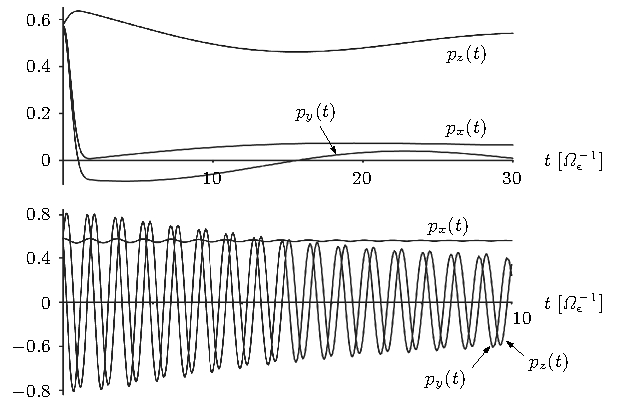
\includegraphics[width=.94\linewidth]{figures/ch05_fig08.pdf}
\caption{Cucchietti、Paz、Zurek\cite{ref118}が調べた、偏極ベクトルの成分$p_x(t)$、$p_y(t)$、$p_z(t)$［(5.166)参照］の時間依存性。このベクトルは、Hamiltonian(5.150)で定義されるスピン・スピン模型の、縮約密度行列の発展［(5.160)参照］を記述する。時間$t$の単位は、系の固有発展の特徴的時間尺度$\Omega_\epsilon^{-1}$である。上は固有動力学が弱い場合（$\Delta_0=0.1s_N$）で、$\hat\sigma_z$の近似的固有状態を優先基底として選ぶ。下は、系の自己動力学が強く、環境モードが低エネルギー、すなわち「遅い」という、逆の状況（$\Delta_0=5s_N$）である。このとき$\hat\sigma_x$、したがって自己Hamiltonianの、近似的固有状態が指針状態として現れる。}
\end{figure}
% 原文 p.228
\hypertarget{srcpage:228}{}\label{srcpage:228}
成分$p_x(t)$と$p_z(t)$の最終値の比は、小さい比$\Delta_0/s_N$と同程度となる。したがって、環境が選ぶ優先的指針状態は、$\hat\sigma_x$からの小さな寄与を伴う、$\hat\sigma_z$固有状態に近いことが分かる。

第二の極限、環境が利用できる最大エネルギーが系のエネルギー間隔$\Delta_0$より小さい、$s_N\ll\Delta_0$の場合を考えよう。対応する偏極成分の発展を図5.8下に示す。$p_y(t)$、$p_z(t)$は、包絡線が急速に減衰する振動を示し、$p_x(t)$は$1/2$に近い定常値へ速やかに落ち着く。このことは、動力学的に選ばれる優先基底が、今度は$x$スピン演算子$\hat\sigma_x$、したがって自己Hamiltonianの固有基底に近いことを意味する。すなわち、動力学は、エネルギー固有状態を系の指針基底として選ぶ。

この模型は、系の自己Hamiltonianと相互作用Hamiltonianの相対的強さに、優先基底が依存することを、よく示す。優先基底は、全Hamiltonianの下で最も頑健な局所基底として現れる。見たように、相互作用Hamiltonianが自己Hamiltonianを支配する量子測定極限、$\Delta_0\ll s_N$では、優先状態は相互作用Hamiltonianの固有状態となり、2.8.1節の可換性基準(2.89)に一致する。逆に、環境モードが「遅く」、$s_N\ll\Delta_0$で、自己Hamiltonianが系の発展を支配すると、優先基底は「局所的」エネルギー固有状態、すなわち自己Hamiltonianの固有状態で与えられる。2.8.2節で強調したように、このデコヒーレンスの量子極限\cite{ref103}は、環境の存在を単に無視することとは等価でない。むしろ、環境はエネルギー固有状態の重ね合わせをデコヒーレンスさせる。

\subsubsectionlink{弱結合極限のスピン環境模型：振動子環境への写像}
系と環境の結合が弱いという仮定の下では、ある環境と相互作用する縮約系の動力学を、等価な調和振動子環境とその系との相互作用として表せる、という注目すべき事実に、すでに各所で触れた\cite{ref211,ref212}。スピン環境の写像を最初に調べたのは、Caldeira、Castro Neto、de Carvalho\cite{ref208}である。

この写像は、振動子環境によって生じる系の動力学が、スピン環境によるものと同一になる、という意味ではないことを強調する。実際、得られる動力学は一般に大きく異なる。むしろ「写像」で伝えたいのは、あるスペクトル密度のスピン環境中での縮約動力学が、元のスピン環境のスペクトル密度を適切に修正したものによって記述される、振動子環境中での縮約動力学と、同一であるという知見である。言い換えれば、
% 原文 p.229
\hypertarget{srcpage:229}{}\label{srcpage:229}
スピン環境のBorn--Markovマスター方程式は、振動子環境のBorn--Markovマスター方程式(5.22)を、修正したスペクトル密度で評価して与えられる。その方法を示そう。

\paragraphlink{模型}
スピン環境模型のHamiltonianを、通常の形に分解する。
\chfiveeq{167}
ここで$\hat H_{\mathrm S}$は、系の一般的な自己Hamiltonianである。環境の自己Hamiltonianも含めた。
\chfiveeq{168}
$\Delta_i$は、第$i$環境スピンのトンネル行列要素である。この自己Hamiltonianは、2.10節と5.4.1節の、より単純なスピン環境模型とは異なり、環境に固有の動力学を与える。簡単のため、各スピンの非対称エネルギーはゼロ、すなわち各環境「粒子」が対称二重井戸ポテンシャル中を動くとする\footnote{非対称エネルギーが非ゼロで、したがって自己Hamiltonian(5.168)に$\hat\sigma_z^{(i)}$に比例する項が含まれる場合も、本節とほぼ同じ方法で扱える\cite{ref242}。}。

最後に、相互作用Hamiltonian$\hat H_{\mathrm{int}}$は通常の形となる［(5.150)と比較］。
\chfiveeq{169}
すなわち、系の一般的座標$\hat s$が、各環境スピンへ双線形に結合し、強度は$g_i$で定量化される。後で、スピン系の$\hat s=\hat\sigma_z$、すなわち「スピン・スピン模型」と、調和振動子系の$\hat s=\hat X$の場合に、特化する。

\paragraphlink{スピン環境の自己相関関数の計算}
弱い系・環境結合の極限を仮定し、環境は温度$T$で熱平衡にあるとする。このスピン浴模型のBorn--Markovマスター方程式（4.2節参照）を導きたい。まず目標となるのは、環境自己相関関数(4.10)の導出である。量子Brown運動の場合［(5.5)と比較］と同じく、相互作用Hamiltonian(5.169)は一項だけを含むので、計算すべき環境自己相関関数は、ただ一つである。
\chfiveeq{170}
% 原文 p.230
\hypertarget{srcpage:230}{}\label{srcpage:230}
ここで$\hat E(\tau)=e^{i\hat H_{\mathrm E}\tau}\hat E e^{-i\hat H_{\mathrm E}\tau}$は、(5.169)で定義した集団的環境演算子$\hat E$を、相互作用描像で表したものである。

環境スピン同士は相互作用せず、したがって$i\ne j$で$[\hat\sigma_x^{(i)},\hat\sigma_z^{(j)}]=0$なので、指数関数$e^{i\hat H_{\mathrm E}\tau}$は、単一スピンの項へ因数分解される。
\chfiveeq{171}
したがって、環境自己相関関数(5.170)は、次と書ける。
\chfiveeq{172}
ここで再び、環境スピンが直接相互作用せず、したがって無相関である事実を使うと、$i\ne j$について、
\chfiveeq{173}
となる。量子Brown運動模型での同様の議論については、(5.7)を比較されたい。したがって、(5.172)の和を分解できる。
\chfiveeq{174}
次に、スピン浴による「量子的力」の平均が$t=0$でゼロ、すなわち、
\chfiveeq{175}
と仮定する。もしゼロでなくても、定数を加えれば常に実現できるので、制限を課す仮定ではない。このことは、(5.174)右辺の最初の和に現れる項$\sum_{j\ne i}g_j\langle\hat\sigma_z^{(j)}\rangle_{\hat\rho_{\mathrm E}}$も、近似的にゼロであることを意味する。これにより$i\ne j$の交差項を無視し、(5.172)を大幅に簡単化できる。
\chfiveeq{176}
最後の行では、浴の初期状態$\hat\rho_{\mathrm E}$についての熱平均を、$Z=\operatorname{Tr}_{\mathrm E}e^{-\hat H_{\mathrm E}/(k_{\mathrm B}T)}$として、明示的に書いた。まず、浴スピンが無相関なので、すべてのスピンを含む初期状態の熱平均は、単一スピンの平均に還元される。
% 原文 p.231
\hypertarget{srcpage:231}{}\label{srcpage:231}
\chfiveeq{177}
ここで$Z_i$は(5.112)と同じ定義である。次に、相互作用描像の演算子$\hat\sigma_z^{(i)}(\tau)$の時間発展を計算する必要がある。
\chfiveeq{178}
$\hat\sigma_z^{(i)}$の固有基底を$\{|\uparrow\rangle_i,|\downarrow\rangle_i\}$とすると、環境Hamiltonian$\hat H_{\mathrm E}^{(i)}$の明示的行列表現は、
\chfiveeq{179}
である。対角化により、固有値$E_\pm=\pm(-\Delta_i/2)$と、固有ベクトル$|\pm\rangle_i=(|\uparrow\rangle_i\mp|\downarrow\rangle_i)/\sqrt2$が得られる。新しい基底$\{|+\rangle_i,|-\rangle_i\}$では、演算子$\hat\sigma_z^{(i)}$は、
\chfiveeq{180}
という形となる。したがって、相互作用描像の時間発展は、
\chfiveeq{181}
である。これらの具体的表式を使うと、(5.177)右辺の波括弧内は、
\chfiveeq{182}
となる。この式のトレースを、簡単のため$\{|+\rangle_i,|-\rangle_i\}$基底で取り、
\chfiveeq{183}
を用いると、環境自己相関関数(5.177)の具体的形が得られる。
\chfiveeq{184}
最後に、通常の手順に従って、環境自己エネルギー$\Delta_i$についての離散和を、スペクトル密度
% 原文 p.232
\hypertarget{srcpage:232}{}\label{srcpage:232}
\chfiveeq{185}
を用いて積分へ置き換える。環境自己相関関数の最終表式が得られる。
\chfiveeq{186}
これが主要な結果である。スピン浴が等価な振動子浴へどう写像されるかを見るため、これを使おう。

\paragraphlink{スピンから振動子への写像}
スピン環境自己相関関数の式(5.186)を、調和振動子浴の場合に得た環境自己相関関数(5.15)、すなわち、
\chfiveeq{187}
と比較しよう。ここで、
\chfiveeq{188}
は、調和振動子環境のスペクトル密度である。スピン浴の場合の対応物と区別するため、添字「osc」を付けた。

(5.186)と(5.187)を比べると、振動子浴で明示的な温度依存性を持っていた雑音核$\nu(\tau)$、すなわち$C_{\mathrm{osc}}(\tau)$の実部は、スピン浴では、その温度依存性を失っている。式(5.186)の$C(\tau)$の実部は、明示的な温度依存性を含まない。他方、スピン浴の$C(\tau)$の虚部には、温度依存因子$\tanh[\Delta/(2k_{\mathrm B}T)]$があるが、$C_{\mathrm{osc}}(\tau)$の対応する散逸核$\eta(\tau)$には、そのような明示的温度依存性がない。

二表式が一致する唯一の場合は、$T\to0$で$\tanh[\Delta/(2k_{\mathrm B}T)]\to1$、$\coth[\omega/(2k_{\mathrm B}T)]\to1$となる、零温度の場合である。これは次のように理解できる。零温度では、それぞれの環境中のスピンも調和振動子も、実効的に基底状態に閉じ込められ、励起状態を占められない。したがって、スピンは二次元状態空間に限られるのに、振動子は連続的なエネルギー準位を占められるという、両者の特徴的な違いが、$T\to0$で消え、浴は同様に振る舞う。

% 原文 p.233
\hypertarget{srcpage:233}{}\label{srcpage:233}
しかし、少し工夫すれば、有限温度でも、スピン浴の式(5.186)を振動子浴の式(5.187)へ写像できる。新しい有効スペクトル密度$J_{\mathrm{eff}}(\Delta,T)$を、
\chfiveeq{189}
で定義しよう。$J(\Delta)$は元のスピン浴のスペクトル密度(5.185)である。環境自己相関関数(5.187)に現れる振動子浴の$J_{\mathrm{osc}}(\omega)$を、明示的に温度依存するこの式$J_{\mathrm{eff}}(\Delta,T)$へ置き換える。右辺の積分で記法を$\omega\to\Delta$と変えると、
\chfiveeq{190}
を得る。これは、まさにスピン浴の環境自己相関関数(5.186)である。

したがって、5.2節で振動子浴について導いた、以前のすべての結果を、スピン浴へ引き継ぐ簡単な道筋が見つかった。浴のスペクトル密度に依存する振動子浴の式を、修正した「代用」スペクトル密度(5.189)で評価するだけでよい。それは、真のスピン浴のスペクトル密度$J(\Delta)$に、追加の温度・周波数依存因子$\tanh[\Delta/(2k_{\mathrm B}T)]$を掛けたものである。

特に、スピン浴の核$\nu(\tau)$、$\eta(\tau)$は、次で与えられる。
\chfiveeq{191_192}
これは、新しい有効スペクトル密度(5.189)を、(5.16)、(5.17)へ代入したものである。これらの核の式と、振動子浴の対応する式(5.16)、(5.17)との形式的な違いは、一見それほど大きく見えないかもしれない。しかし、縮約動力学への影響は、非常に大きくなり得る。写像の手順を、二つの具体例で調べよう。

\paragraphlink{例1：スピン・スピン模型からスピン・ボソン模型への写像}
中心系を、$\hat\sigma_z$を介してスピン浴へ双線形に結合する、スピン$1/2$粒子で表す場合を考える。
% 原文 p.234
\hypertarget{srcpage:234}{}\label{srcpage:234}
上の写像法によれば、量子Brown運動のマスター方程式の一般表式(5.22)で、$\hat X\to\hat\sigma_z$と代入すれば、Born--Markovマスター方程式を直ちに書き下せる。
\chfiveeq{193}
核$\nu(\tau)$、$\eta(\tau)$は、今やスピン浴の式(5.191)、(5.192)で与えられる。

スピン・ボソン模型の議論（5.3.2節参照）と同じく、系の自己Hamiltonianを$\hat H_{\mathrm S}=-\frac12\Delta_0\hat\sigma_x$とすると、相互作用描像の演算子$\hat\sigma_z(\tau)$の明示的時間発展は、
\chfiveeq{194}
となる。これを(5.193)へ使うと、マスター方程式
\chfiveeq{195}
が得られる。この方程式は、スピン・ボソンのマスター方程式(5.142)と、形式的に同一である。これはもちろん意外ではない。目標は、スピン浴を、等価な振動子浴、すなわちボソン浴へ写すことであった。(5.195)に現れる量の定義は、スピン・ボソンの場合と同じ［(5.143)、(5.144)、(5.145a)参照］だが、核(5.191)、(5.192)で評価する。

\paragraphlink{例2：振動子・スピン模型から量子Brown運動模型への写像}
写像法のもう一つの例として、中心調和振動子がスピン浴へ弱く結合する場合\cite{ref242}を論じよう。この弱結合「振動子・スピン模型」は、6.4.2節で詳しく論じる、量子電気機械系のデコヒーレンスと散逸の模型化へ、応用できる可能性がある。全Hamiltonian
\chfiveeq{196}
で記述される、かなり一般的な振動子・スピン模型を考える。ここで、
\chfiveeq{197}
% 原文 p.235
\hypertarget{srcpage:235}{}\label{srcpage:235}
は、中心系の固有動力学を表す通常の調和振動子Hamiltonianである。環境の自己Hamiltonian$\hat H_{\mathrm E}$は、おなじみの形(5.168)を持つ。相互作用Hamiltonian$\hat H_{\mathrm{int}}$は、中心振動子の位置座標と、各環境スピンの$z$スピン座標との双線形結合を表す。

再び、弱結合極限が適用されると仮定し、スピン浴から振動子浴への写像の方針に従えば、振動子系の縮約動力学を、調和振動子ポテンシャルに閉じ込めた粒子の、量子Brown運動のBorn--Markovマスター方程式(5.25)で、容易に記述できる。
\chfiveeq{198}
周波数シフト$\widetilde\Omega^2$、運動量減衰率$\gamma$、拡散係数$D$、$f$は、量子Brown運動と同じ表式(5.26)で与えられる。ただし、そこに現れる核$\nu(\tau)$、$\eta(\tau)$は、「代用」スピン浴の核(5.191)、(5.192)へ置き換える。

スピン浴のオーム型スペクトル密度の例を考えよう。
\chfiveeq{199}
これは、量子Brown運動の文脈で考えた、オーム型密度(5.44)と形式的に同一である。5.2.3節で詳述した方法に従い、スペクトル密度の具体形を選ぶと、マスター方程式(5.198)の係数を評価できる。

以前と同様、係数$\gamma$、$D$は、それぞれ二重Fourier正弦変換、余弦変換で与えられる。詳細は5.2.3節の議論を参照されたい。したがって、結果の式を容易に書き下せる［(5.46)、(5.48)と比較］。
\chfiveeq{200_201}
オーム型振動子浴とは対照的に、オーム型スピン浴では、運動量減衰係数$\gamma$が明示的に温度依存する。因子$\tanh[\Omega/(2k_{\mathrm B}T)]$、したがって$\gamma$は、温度が高まると減少する。これは一見、かなり直観に反するかもしれない。「暖かい」環境は、系へより強く影響するか、少なくとも「冷たい」環境より弱い減衰を誘起することはない、と予想するからである。
% 原文 p.236
\hypertarget{srcpage:236}{}\label{srcpage:236}

しかし、この減衰係数の温度依存性は、かなり容易に説明できる。振動子浴では、各振動子は無限個のエネルギー準位を持つため、浴が吸収できるエネルギー量に上限がない。対照的に、スピン$1/2$粒子は二準位しか持たないので、温度、したがって系から吸収できるエネルギー量が高まると、スピン浴全体が非常に速く飽和する。量子Brown運動模型の振動子浴の散逸率は温度に依存しない［(5.46)参照］から、スピン浴が系へ散逸的効果を及ぼす能力は、温度の上昇とともに低下しなければならない。実際、(5.200)が予測する減衰率の温度依存性は、フォノン、すなわち振動子モードと二準位系の相互作用によって散逸が起きる\cite{ref245}、ガラスのような物理系で実験的に観測されている\cite{ref244}。

オーム型スピン浴では、通常拡散係数(5.201)、したがって空間的デコヒーレンス率は、明示的な温度依存性を持たない。これは、$\coth[\Omega/(2k_{\mathrm B}T)]$に従い、環境温度が高いほど空間的デコヒーレンスが強まる、量子Brown運動の通常拡散係数(5.48)と対照的である。実際、Caldeira--Leggett模型の高温極限では、$D$が温度に線形に増すことが分かった［(5.51)参照］。

この違いもまた、各環境粒子が利用できる状態空間の大きさから理解できる。温度とともに、環境振動子が、ますます高く励起された多くの準位を占められることは、環境中の特徴的波長が、ますます短くなることにつながる。典型的環境波長が短いほど、中心系の位置をよく分解でき、得られる経路情報が増すため、空間的デコヒーレンスが強くなる（5.2.6節の議論も参照）。

これに対して、スピン$1/2$粒子が占められるのは二準位だけである。典型的環境波長の範囲、したがって空間的デコヒーレンス率は、温度を高めると非常に速く飽和する。この特定の模型では、それは完全に温度に依存しない率さえもたらす。実際、この模型では環境二準位系が対称二重井戸ポテンシャル中を動くと仮定した。したがって、対応するスピン粒子の二状態は同じエネルギーに結びつけられ、状態空間をさらに制限する。この対称性の仮定を捨て、浴Hamiltonianへ$\sum_i(\omega_i/2)\hat\sigma_z^{(i)}$という非対称項を含めると、空間的デコヒーレンス率に、定数ではあるが、依然として温度非依存の値が加わることを、容易に示せる。この増加は、浴粒子が利用できる状態空間が広がったことを反映し、
% 原文 p.237
\hypertarget{srcpage:237}{}\label{srcpage:237}
それは、より短い環境波長の存在に対応する。

\subsubsectionlink{Markov近似を超えて：一般のスピン環境模型を解く}
最後に、制限的なBorn--Markov近似へ頼らずに、より一般的なこの種の模型をどう解けるか、簡単に示して、スピン環境模型の議論を終えよう。5.1.2節で論じたように、この模型で興味深いのは、通常、低温かつ系・環境結合が強い領域である。このとき、環境には有意な非Markov記憶効果が生じ、簡単化する弱結合近似は通常使えなくなる。したがって、前の5.4.2節で行ったような、弱結合と無視できる環境自己相関時間を基礎に導かれる、近似的なBorn--Markovマスター方程式で扱えないことが多い。そのため、このような非Markovスピン環境模型の数学的解法は、しばしばやや複雑になる。

多くの場合、一般的なスピン環境模型から生じる、たとえば中心スピンの期待値$\langle\hat\sigma_z(t)\rangle$に関する、関係するデコヒーレンス動力学は、インスタントン形式\cite{ref199}などの高度な手法で解析的に計算できる。このとき、強く結合したスピン環境の自由度を、どう適切に「平均」するかが問題となる。Prokof'evとStamp\cite{ref199}は、一般的模型を四つの極限へ分けることで、これを容易にできることを示した。各極限は異なるパラメーター領域を重視し、全Hamiltonianの一般表式の特定の項を捨てる。それぞれを別々に解くと、模型のある量についての平均積分の式が得られる。\cite{ref199}で示されたように、一般の場合にスピン環境を平均し、したがって中心系の縮約動力学を得る正しい手順は、これら四つの別々の平均を、組み合わせて適用するだけで与えられる。ここでは詳細には立ち入らず、関心のある読者には\cite{ref199}を案内する。スピン環境模型の物理的・数学的基礎についての、さらなる議論は、\cite{ref200,ref210,ref214,ref216}にある。
